
\section{Study Design}
\label{sec:study}

% TODO Caro: I find this figure still very confusing :'(, due to a lack of structure. If you want me to, I can give it a go?
\begin{figure*}[tb]
	\centering
	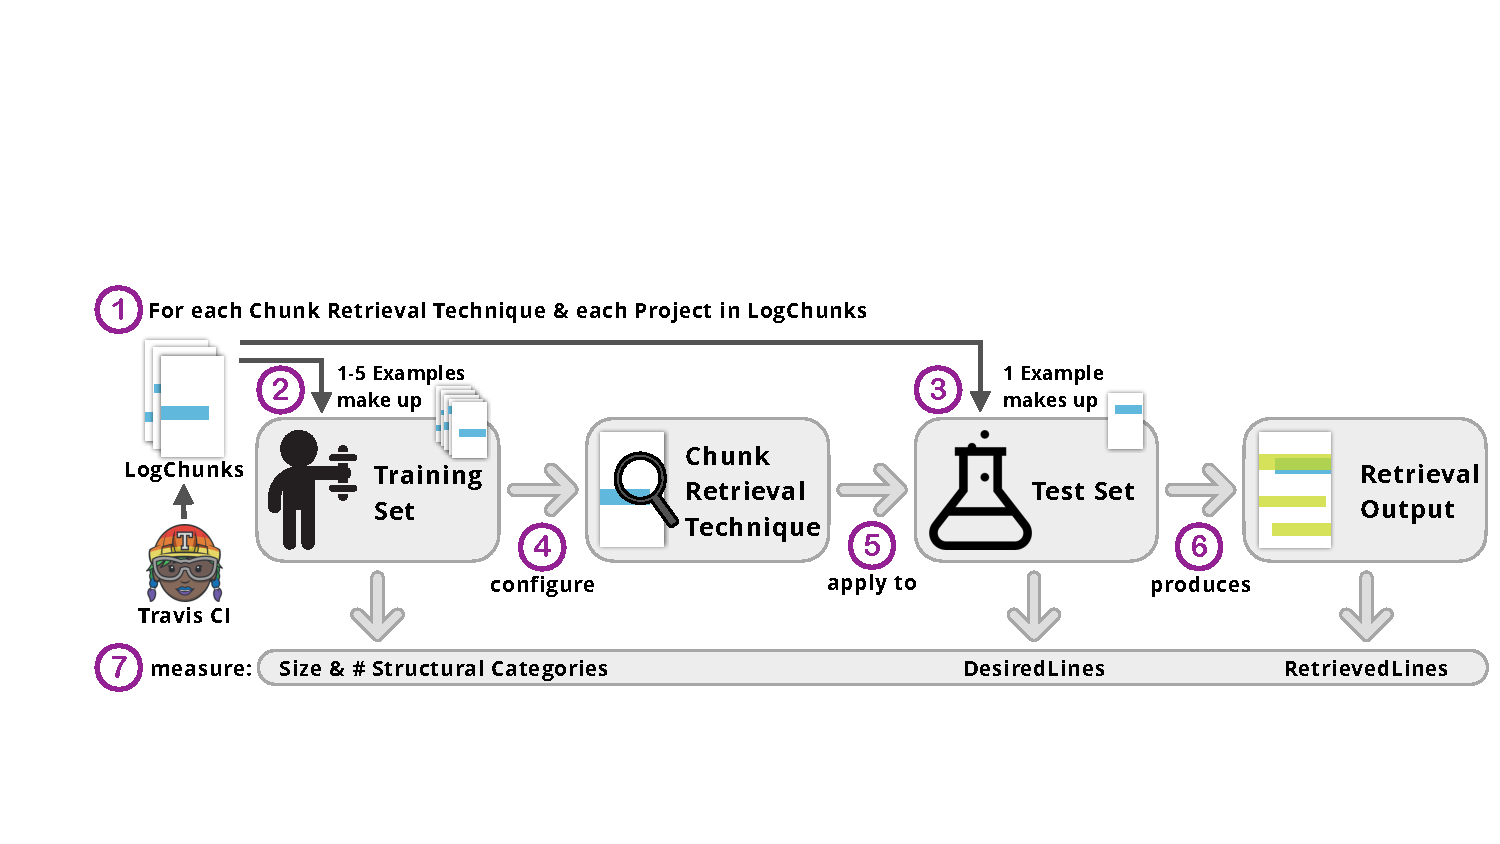
\includegraphics[width=\textwidth, trim={0.4cm 8.4cm 1.2cm 0.3cm}, clip]{img/study.pdf}
	\caption{Study design of our technique comparison study.}
	\label{fig:study}
\end{figure*}

To investigate which techqnique is best suited to retrieve chunks from
CI build logs we evaluate them on the
\emph{LogChunks}~\cite{brandt2020logchunks} data set. This section
describes our study design and which metrics we measure to answer our
research questions. In the presentation of the results, we first focus
on each of the three techniques and later compare them against each
other.

\subsection{LogChunks}
For this study we created the previously published data set
\emph{LogChunks}. It encompasses 797 build logs from Travis CI,
stemming from a broad range of 80 GitHub repositories and 29
programming languages. For each file, the authors manually ``labeled
the log part (chunk) describing why the build
failed''~\cite{brandt2020logchunks}. We include keywords, which we
would use to search for the selected chunk within the log. In
addition, we categorized the log chunks according to their format
within the log. If the chunks are surrounded by the same markings
within the log we assign them the same structural category.

For the comparison, we evaluate the three chunk retrieval techniques
PBE, CTS and KWS, described in Sections~\ref{sec:expl-pbe},
\ref{sec:expl-ts} and \ref{sec:expl-skws}. Random Line Retrieval
(RLR), explained in Section~\ref{sec:expl-rlr}, acts as a baseline for
the comparison.
% We run four techniques on the examples from \emph{LogChunks}.

\noindent
\textbf{Training and Test Set}
We use \emph{LogChunks} as the data set for our study. For each of the
80 repositories in it, \emph{LogChunks} contains 10 build logs,
manually labeled with the \emph{chunk} describing the
reason the build failed. Additionally, it contains (1) keywords useful
to identify the substring in the log  and (2) which structural category
the substring belongs to.
% TODO Moritz: You said: Add details how key words were extracted. Add example?
% how the keywords were put in logchunks does not fit here, that is
% maybe answered 2 paragraphs above already?
% how KWS uses the keywords is already described in the section
% introducing the technique => I would scrap everything but the first
% sentence directly above here :)

% TODO Moritz: You said: Add more details. How was the split in numbers?
% this is described in the following paragraph, should we merge them
% (bc there are also no sub-RQs now) or is it close enough? :)
For each repository in \emph{LogChunks}, we split the examples
chronologically into training and test set. Therefore, we train on
examples from past build logs and test on more recent build logs.

\noindent % TODO: adapt if we change the research questions
\textbf{RQ 2.1: Size of Training and Test Set}
To analyze how many examples the chunk retrieval techniques need to
perform best, we evaluate the techniques with different training set
sizes. We train each technique with one to five examples from each of
the repositories within \emph{LogChunks}. The size of the test set is
one.

\noindent
\textbf{RQ 2.2: Recording Structural Categories}
To determine how structurally similar the examples for the chunk
retrieval techniques need to be, we record the structural categories
of the examples in the training and test sets.

\noindent
\textbf{RQ2.3: Accuracy Metrics}
To measure the accuracy of the retrieved chunks we save the output
lines of the chunk retrieval run on the input of the test example
($\mathit{RetrievedLines}$). As oracle in our evaluation, we save the
desired lines from the output of the test example
($\mathit{DesiredLines}$).

We calculate and define a number of metrics for the context of our
evaluation.

\vspace{0.2cm}
\begin{itemize}[leftmargin=0.4cm] \itemsep1em
	\item $|\mbox{True positives}| = \mathit{DesiredLines} \cap
	\mathit{RetrievedLines}$ \vspace{0.2cm}\\
        True positives are lines that appear both in the output of a
        tool as well as what \textit{LogChunks} contains for each
        example. 
        % What about when a line is replicated twice?
        % I.e., Are line numbers part of this? => no.
        % not checked, but if lines are identical they also contain
        % the same information so if someone asks we can defend I think
	\item $\mbox{Precision} = \dfrac{|\mathit{True\
	Positives}|}{|\mathit{RetrievedLines}|}$ \vspace{0.21cm} \\
        Precision of a chunk retrieval describes which proportion of
        the retrieved lines were actually desired. 
	\item $\mbox{Recall} =
	\dfrac{|\mathit{TruePositives}|}{|\mathit{DesiredLines}|}$
	\vspace{0.2cm} \\
        Recall of a chunk retrieval describes which proportion of the
        desired lines were retrieved.
	\item $\mbox{F$_{1}$-score} = 2 \cdot \dfrac{\mathit{Precision}
	\cdot \mathit{Recall}}{\mathit{Precision} + \mathit{Recall}}$
	\vspace{0.2cm}\\
        In addition, we calculate the F$_{1}$-score, the harmonic mean
        of precision and recall. We prefer F$_{1}$ to other aggregate
        measures such as accuracy because for a
        ``needle-in-the-haystack'' scenario, we do not want to bloat
        our results by correctly not finding lots of irrelevant log
        lines.
	\item Successful retrieval = $\mathit{true}\ \mathit{iff}\
	\mathit{Recall} = 1, \mathit{false\ otherwise}$  \vspace{0.2cm} \\
	We define a successful retrieval as one where all desired lines were
	extracted, therefore when recall is one.
\end{itemize}

% Recall and precision of CTS and KWS vary with the number of lines
% selected for retrieval. We evaluate the effect of varying the number
% of extracted lines by multiplying the average number of lines
% present in the training examples with a \emph{retrieval size factor}
% from 0.5 to 2.5 in steps of 0.5.
